\documentclass[12pt, twoside]{report}
\usepackage[a4paper,width=150mm,top=25mm,bottom=25mm,bindingoffset=6mm]{geometry}
\usepackage{graphicx}
%\usepackage{fancyhdr}
\usepackage{scrextend}
\usepackage{amsmath}
\usepackage{blindtext}
\usepackage{enumitem}
\usepackage{array}
\usepackage{multirow}
\usepackage{rotating}
\usepackage{tikz}
\usepackage{etoolbox}
\usepackage{hyperref}
\graphicspath{ {Images/} }
\addtokomafont{labelinglabel}{\sffamily}

\patchcmd{\thebibliography}{\chapter*}{\section*}{}{}

\title{
    {Firecode Receiver for Small Satellite Systems}\\
    {\large McGill University}\\
    {\small Advised by Frank F. Ferrie}\\
    {\small In Association with \textbf{Aquila Space, Inc.}}\\
}
\author{Derek Yu, \textit{260570997}\\ Markus Suorsa, \textit{260551931}}
\date{ 30 March 2016}

\begin{document}
\maketitle

\chapter*{Abstract}

\par With Moore's Law as a major driving force behind the development of electronics, the small satellite industry has been able to take advantage of lower payload costs, increased miniaturization, faster development, and experimental technologies to implement continuous deployment strategies.
As a result, the probability is high that satellites will encounter glitches, usually of the software variety, that may render the spacecraft inoperable.
In order to re-establish communication to fix these issues and resume operation, an independent system to reset all spacecraft systems is required.
Markus Suorsa and Derek Yu of McGill University, with association with Aquila Space, are developing the FRS3 (Firecode Receiver for Small Satellite Systems) as a possible solution.
The FRS3 is an open source project with a small footprint, and a configurable setup for many different applications.
It will take the form of a PCB and antenna acting as an independent system upon a spacecraft.
The FRS3 will be using a low-power Nominal Operation with periodic sleep-RX cycles and an Active Operation for decrypting unique signals before emitting the reset signal to the rest of the spacecraft.
This semester was primarily focused on research on topics such as RF communication/components, and designing the system architecture and interconnections between major components, as well as creating the theory of operations.
This was accomplished with personal research and regular guidance from industry experts at Aquila Space.


\chapter*{Acknowledgements}
Thank you to Kyle Leveque, Gordon Hardman, and Jan King, and all of Aquila Space for their guidance in this project. Also thank you to our supervisor, Professor Frank Ferrie for his insight and review.

\chapter*{List of Acronyms}
\begin{labeling}{FCC}
\item [\textbf{CSA}] Canadian Space Agency
\item [\textbf{ESA}] European Space Agency
\item [\textbf{FCC}] United States Federal Communications Commission
\item [\textbf{FRS3}] Firecode Receiver for Small Satellite Systems
\item [\textbf{GEO}] Geosynchronous Earth Orbit
\item [\textbf{IC}] Integrated Circuit
\item [\textbf{LEO}] Low Earth Orbit
\item [\textbf{NASA}] National Aeronautics and Space Administration
\item [\textbf{PCB}] Printed Circuit Board
\item [\textbf{RCM}] RADARSAT Constellation Mission
\item [\textbf{RF}] Radio Frequency
\item [\textbf{SAR}] Synthetic Aperture Radar

\end{labeling}

\addtocontents{toc}{\protect\enlargethispage{2\baselineskip}}
\tableofcontents

\chapter{Motivation}
\par With continuing advancements in technology, two things tend to change.
First, technological performance increases, providing greater functionality at cheaper costs.
Second, the size decreases, allowing the profile and footprint of devices to shrink.
This is the phenomenon behind Moore's Law.
Although primarily directed towards the semiconductor industry, the idea is applicable to many different fields of engineering.
However, until recently, the satellite aerospace engineering industry has resisted such change, instead opting to continue using outdated yet reliable technology to decrease the risk of using newly developed, potentially volatile systems on multi-million dollar satellites.
Many base components and systems found on satellites launched in the 90's and 00's are exactly the same as those in the 70's and 80's.
Recent developments in the satellite and launch industries have introduced much cheaper platforms for payloads and launches, decreasing the cost involved in satellite development significantly.
As a result, more and more satellites are testing more experimental components.
The risk involved in using these components are less threatening than before, as launch and integration costs have decreases due to smaller satellite platforms.
However, the risk still does exist, and because launch costs are still considerable, there must be a contingency in place to mitigate the risk.

\par In the last decade or so, design paradigm has shifted from a hardware-based approached towards a software-based approach.
New and experimental technologies are heavily software based, while the hardware aspects are similar to older iterations with only marginal changes.
Thus, when issues arise on spacecraft in orbit, they are much more likely to be software-based than hardware-based.
Fortunately, software-based issues may be fixable post-launch, but this varies on the nature of the problem.
Fixes may be uploaded to the spacecraft during a ground pass (please refer to the background for further reading), but if the spacecraft is otherwise unresponsive, it is impossible.
To resume nominal operation and regain communication, a simple power cycle or reset would be sufficient.
However, due to the unfortunate location of a spacecraft in orbit, it is simply not practical to send a person up to hit a reset switch.
It is possible to program the spacecraft to reset all systems at the reception of a particular radio message, but it would not work if the flight computer is unable to process it, or if the communication system is the source of the problem.
If there were a dedicated, independent system which would listen for such a message to reset the spacecraft and be able to do so despite the state of the rest of the spacecraft, than such a product would be inevitable.
This is the idea behind this paper's topic.

\par A need for an emergency reset receiver can be clearly illustrated in the LightSail-1 mission.
In 2015, the Planetary Society launched a CubeSat containing an experimental solar sail into orbit, with its primary mission objective to test the solar sail deployment module.
The satellite was in the 3U CubeSat format and was developed by Stellar Explorations.
Two days after launch, the spacecraft suffered a debilitating software glitch that rendered it unresponsive~\cite{lightsailglitch}.
For several weeks, LightSail remained inoperable until a `natural reboot' occurred, in which the spacecraft was reset by a charged particle in space hitting the electronics in just the right way to force a reboot.
Afterwards, the software was updated from the ground and LightSail was fortunately able to complete its mission.

\par Although the LightSail-1 mission was ultimately successful, there was a period where the recovery of the satellite was in question. When any mission goes awry as a result of technical problems, it is not proper to rely on the occurrence of a `natural reboot' like how LightSail did. If LightSail did contain an emergency reset receiver, as soon as it was clear that the satellite was unresponsive, the team on the ground could have emitted the reset signal to the satellite. The receiver would have received the signal and promptly rebooted the satellite, eliminating the problem.

\chapter{Background}
This section details some areas which may be of relevance regarding the development and context for the FRS3. This is by no means an exhaustive list, and are limited in their scope.

\section{Low Earth Observation and Applications}
\par The two most popular orbits for earth-orbiting spacecraft are Geosynchronous Earth Orbits (GEO) and Low Earth Orbits (LEO).
GEO satellites exist in an altitude of about 36,000km at which its orbital period matches that of Earth's rotation, effectively placing it above constant location on Earth.
This is common for telecommunication satellites and less common for remote sensing.
If a satellite is said to be in LEO it means that it is at altitude of 200–2000km above sea level.
LEO satellites travel in fast orbits across Earth, with the average orbital period of within a couple of hours.
This makes LEO satellites an attractive option for earth observation platforms, particularly if placed in a polar orbit.
In such a configuration, a spacecraft could eventually image the entire surface of Earth.
Satellite constellations such as Canada's RCM, and ESA's Sentinel program are used to gather scientific data about the surface of the earth, with notable applications being surface sea temperatures, area covered by rain-forest, and the thickness of polar ice caps.


\section{The CubeSat Platform}
\par Miniaturized satellite platforms vary in size and weight, ranging from `small satellites' (100–500kg) to `femtosatellites' (10–100g).
The CubeSat platform populates this scale.
CubeSats are made up of units `U' to mean one litre of useful space in a \times10\times10\times10cm$^3$ package.
Smaller CubeSats are of the 1U variety, whereas typical CubeSats are around the 3U+ range.
This smaller size means that costs are kept low in a field where the average cost of delivery into space ranges from millions for small payloads to billions for larger satellites.


\section{Common Satellite Operations}
\par Satellites travel in trajectories across the surface of the earth in orbits, with each time they travel over the same location considered a ground pass.
Due to the curvature of the earth and their low orbit, they generally have a visual range of a few hundred kilometers, in which they are also in communication with a ground station.
This small visual range (compared to the size of the earth) couple with the relative speed at which it travels, means that satellites are only in contact with a base for minutes between passes.
While this makes communication difficult, it means that a satellite can traverse a huge amount of area and collect impressive amounts of data.


\section{RF Communications in Space}
\par Due to the nature of the distance between receiver and the sender, communications in space are typically done at a high frequency, ranging from hundreds of MHz to tens of GHz.
The transmission intensity from the ground station to the satellite (uplink) or from the satellite back down to earth (downlink) must be high enough to be able to take into consideration all the disturbances-the directionality, gain of the antenna, the direction of the ground satellite, the Doppler effect when the satellite is approaching versus travelling away, even the condition of the weather such as clouds and particulates in the atmosphere! Units of this intensity are generally given in decibels (dB) which are defined by the formula:

\begin{equation}
    10\log(\frac{p}{p_0})
\end{equation}

Where the $p$ is the power by the system and $p_0$ is some reference power, generally one Watt. This logarithmic scale makes it more convenient to discuss changes in power. An important reference is that a drop of about 0.3dB is equivalent to a drop in half of the transmitted power. This power plays a key role during calculations of communication both the \textit{power flux density} (or in specific cases, called \textit{intensity}) and then \textit{bandwidth}. The power flux density is the strength of the signal that hits the antenna array. The bandwidth is the range of frequencies for which the signal can be heard.

\par Keeping track of the variables which could affect the gain and the bandwidth are put together in a document commonly known as the link budget.

\chapter{Requirements}~\label{Requirements}
The requirements for the FRS3, aside from those already imposed upon any hardware going into space, was that it had to be reliable. The FRS3 was designed to be used in a last-case scenario, which in itself assumed that critical components were already in a state of emergency. All of the requirements were in line with Occam's Razor (the principle of least complexity) in order to minimize variables which could reduce the reliability of the component. Below are the other high level technical requirements.

\section{Adaptability}~\label{Adaptability}
\par To increase the impact of the FRS3, the subsystem should be compatible with most kinds of spacecraft, from different clients. As such, it needs to  easily interface with many different components. These can be split into two different categories of adaptability: Software flexibility, which focuses more on the reset key, and the cool-down time, which is simply a variable, and hardware adaptability, which includes how the system integrates with elements such as the power bus, and how the reset signal is connected to other components.

\section{Self Contained}
\par Since an emphasis is placed on a system being adaptable for many clients, it must be independent. In addition, because of the nature of the FRS3 being failsafe subsystem, it must be assumed that Murphy's Law is applicable. In this context, it is clear that if such a catastrophe were to occur, the variables which guarantee a successful operation will be prioritized. In this manner, such a device who's primary goal is reliability must also be self contained.

\section{Open Source}
\par Given the nature of the design project, and the products adaptability with various other spacecraft vendors, it seems natural that in order to have the most optimal exposure and longevity of the project, that that product must be entirely open source. Furthermore, all tools and components should also be open source.

\section{Small Footprint}
\par Given that space constrains on current CubeSats are small, it makes commercial sense to have every single component be as compact as space-efficient as possible. Since the FRS3 would mark a non-essential component, it has to be such a product have minimal interference with existing spacecraft components. The goal is for the FRS3 to fit within a packed 1U satellite, which would indicate that it could fit within the typical 3U enclosure.

\section{Low Power}~\label{Low Power}
\par Low power usage is one of the most important aspects when it comes to the functionality. Having a device which can operate for extended periods of time opens applications for using a battery to remove power dependency from other components on the spacecraft.

\chapter{Design and Results}
It must be noted here that the some of the results obtained through the design research phase. As such, the topics presented below are intended to give a broad overview of the research design phase completed this semester.

\section{Frequency}

\par The UHF Band was selected as the primary frequency used. This is because the band, which ranges between 400–470MHz is commonly used for satellite telemetry data as well as being a popular amateur radio frequency. This reduces the amount of legal red-tape needed to test the RF Transceivers that have been acquired. Specifically, the decision was made to have the frequency at 433MHz since this frequency band is unlicensed in North America. Elsewhere, this frequency band is primarily used in amateur radio operations.

\section{RF Transceiver}
\par A critical component of the project would be the choice of transceiver; without one which can fulfill the requirements in Chapter~\ref{Requirements}, the system cannot act on signals which it has received. Therefore this is where a significant effort was made. Criteria used to determine eligibility were as follows:

\begin{itemize}[noitemsep]
\label{RFCriteria}
\item AES Capability
\item Power Consumption (through Standby Current)
\item Data Rate
\item Evaluation board
\item Cost per Unit
\item Ease of Use
\item Footprint
\item Software Challenges
\end{itemize}

The selection process used Table~\ref{tab:RFTransceiver} to determine which of the receivers would be chosen. Using the matrix decision table, The STMicro SPIRIT1, and the OnSemi AX8052151 were selected.

\begin{table}[h!]
\caption{Transceiver Selection}
\centering
\label{tab:RFTransceiver}
\begin{tabular}{ p{3cm} p{2.3cm} p{2.3cm} p{2.3cm} p{2.3cm} }
 \toprule
 \multicolumn{5}{|c|}{Transceiver Data} \\
 \toprule
Transceivers        & SPIRIT-1 & NRF905 & SI4455 & AX8052F151\\
\midrule
 AES                & 128 bit & No & No & No\\
 Sensitivity        & -118dBm & -100dBm & -116dBm & -116dBm\\
 Standby Current    & 600nA & 32uA&  50nA & 40nA\\
 Channel Spacing    & 12.5kHz & 100kHz & 100kHz & 100kHz\\
 Data Rate          & 1–500kbps & 50kbps & 500kbps & 1–600kbps\\
 Eval Board         & Yes & Yes &  No & Yes\\
 Cost per Unit      & \$80 & \$506 & \$210 & \$290\\
 \bottomrule
\end{tabular}
\end{table}

\section{Theory of Operations}
The functionality of the FRS3 can be subdivided into two main areas: pre-launch and post-launch. Pre-Launch concerns itself with regards to the flexibility aspect mentioned in Section~\ref{Adaptability}, whereas post-launch can be further subdivided into two main categories to preserve power: Nominal Operation, and Active Operation.

\subsection{Pre-Launch}
Configurations need to be able to be made in two main areas, software and hardware. By being able to partition the two, the client is able to acquire flexibility and compatibility with existing spacecraft systems.

\begin{figure}[h]
\caption{Pre-Launch Operation}
\centering
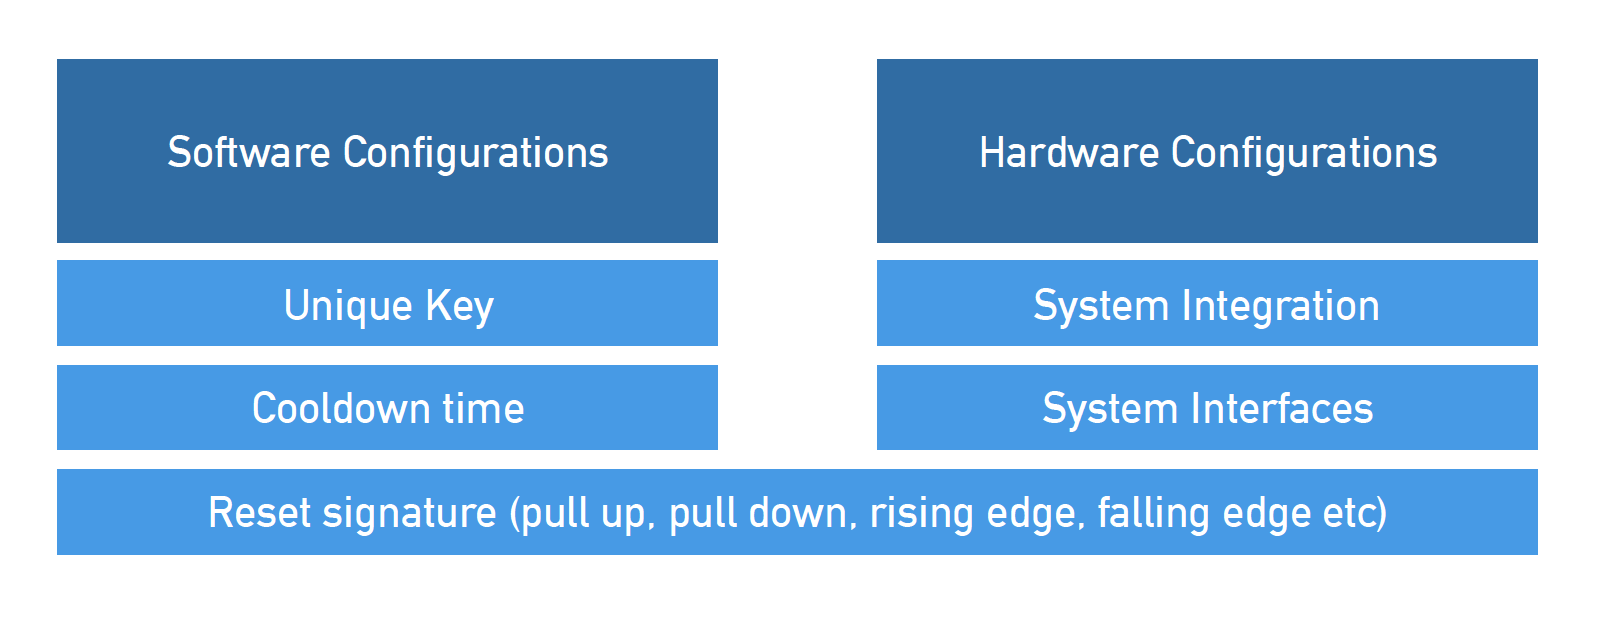
\includegraphics[scale = 0.4]{Pre_Launch}
\end{figure}

\par The reset signature (not the reset/unique key) is the pulse which is emitted by the FRS3 after successful confirmation of the unique key. In this way, it is the method in which the FRS3 interfaces with the necessary systems during Active Operation detailed further in this report.

\subsection{Nominal Operation}
In order to fit within the power consumption constraints outlined in~\ref{Low Power}, a Nominal Operation mode had to be established. A trade-off had to be made between power consumed in receive (RX) mode and in sleep mode, and the time spent. By having a sleep-cycle in nominal operation, the average minimum power usage decreases while still being able to receive messages.
\newline

\begin{figure}[h]
\caption{Nominal Operation}
\centering
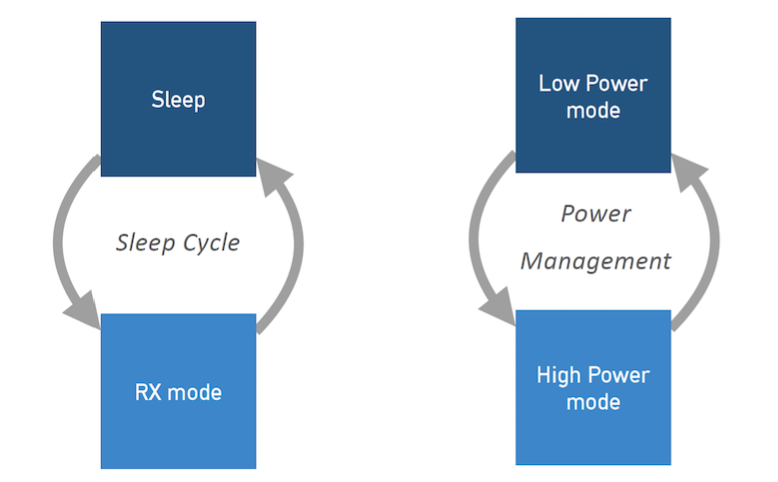
\includegraphics[scale=0.7]{Nominal_Operation}
\label{Nominal_Operation}
\end{figure}

\par Looking at the above Figure~\ref{Nominal_Operation} together with Table~\ref{tab:power_table} it can be seen that RX mode consumes orders of magnitude more than sleep.

\begin{table}[h]
    \centering
    \begin{tabular}{c c}
         State & Current Consumption \\
         \toprule
         SHUTDOWN & 0 \\
         READY & 400$\mu$A \\
         LOCK & 4.4$m$A \\
         RX & 9.2$m$A \\
         SLEEP & 850$n$A
    \end{tabular}
    \caption{Current Consumption of Different States of the SPIRIT1}
\label{tab:power_table}
\end{table}

In its most minimal state, it can be seen that the average power consumption can be derived using the following formula:

\begin{equation} \label{eq:power_consumption}
    \begin{split}
    P_{average} &= T_{RX}P_{RX} + T_{sleep}P_{sleep} \\
    T_{RX} &= M_{length}N_{messages}D_{rate} \\
    T_{sleep} &= 60-T_{RX}
    \end{split}
\end{equation}

\par There are several assumptions associated with these preliminary calculations:

\begin{itemize}[noitemsep]
\item Instantaneous change from RX to SLEEP
\item RX can receive at $D_{rate}$ without bit loss
\item RX will be able to `lock on' to uplink frequency
\item RX can `lock on' within one message of $M_{length}$ length
\item Decryption in RX is instantaneous
\end{itemize}

\par By using these assumptions, we can determine that:

\begin{equation} \label{eq:power_consumption_numerical}
    \begin{split}
    T_{RX} &= (100b/msg)(3msg)(1kbps) \\
    T_{sleep} &= 60s-0.3s \\
    I_{average} &= (0.3s)(9.2mA) + (59.7s)(850nA) \\
    I_{average} &= 1.31 \mu A $/min$ \\
    \end{split}
\end{equation}

Given that the voltage in spacecraft generally varies between 2–12V, the FRS3 should still be operating at a power consumption rate in the range of $\mu W$.

\subsection{Active Operation}
If the signal is detected during the Nominal Operation, the FRS3 goes into Active Operation.

\begin{figure}[h]
\caption{Active Operation}
\centering
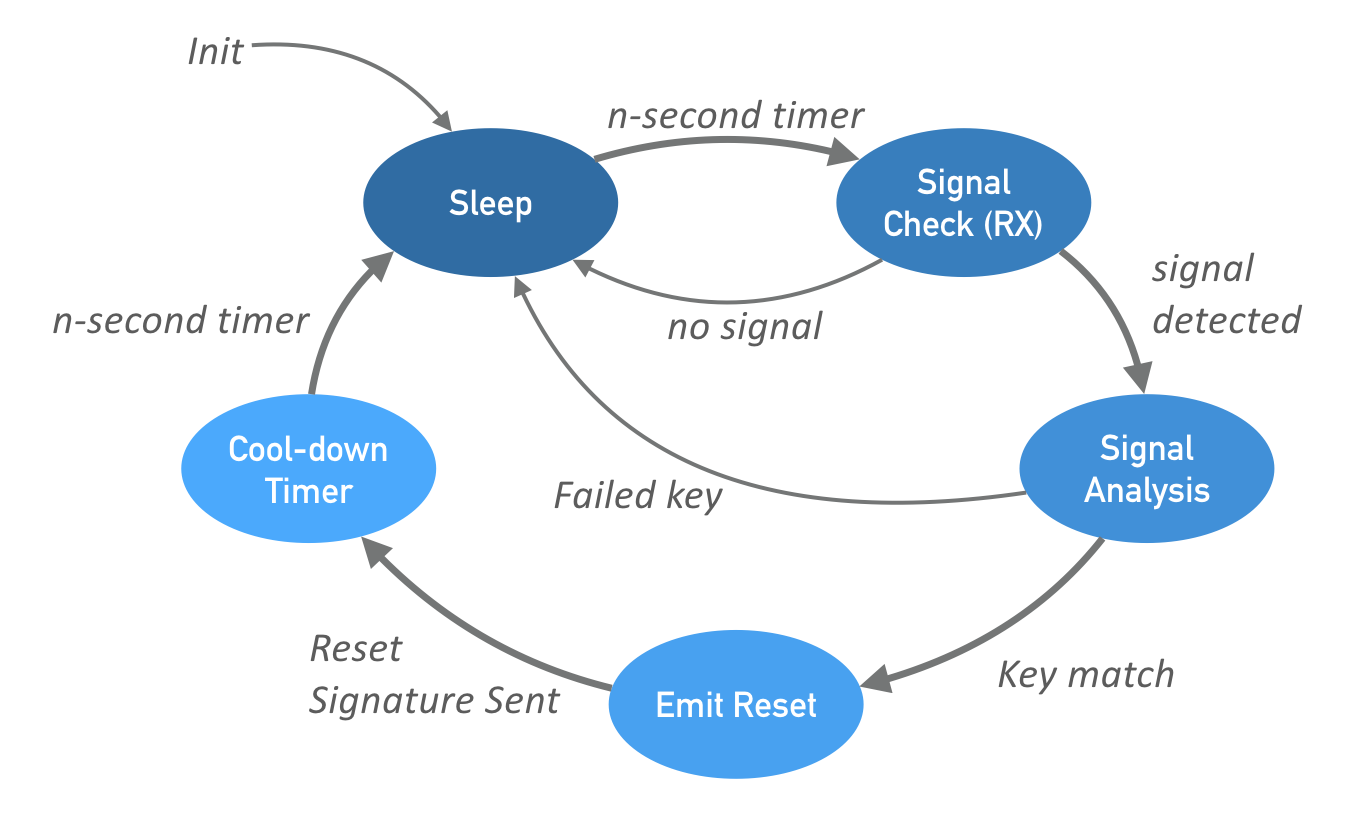
\includegraphics[scale=0.5]{Active_Operation}
\label{Active_Operation}
\end{figure}

In this manner, the sleep and the signal check form the basis of the Nominal Operation. Beginning from Signal Analysis, all the way to the end of the cool-down timer, the system is in Active Operation.

\section{Power System}
Power delivery is another component of the FRS3 that demands attention; insufficient power delivery will harm the functionality through potential blackout, brownout, or decreased lifespan through inconsistent power delivery. Through the research design phase, key elements have been identified as being of importance:

\begin{itemize}[noitemsep]
\label{Power_Delivery_Requirements}
\item Able to support sustainable battery in orbital parameters
\item Able to charge from the main power bus during non-critical operation
\item Powers FRS3 using battery when main power bus is offline
\item Supports current pulsing for optimal FRS3 operation
\end{itemize}

\chapter{Plan for Next Semester}
\par The majority of the first semester was spent on research and learning, while the second semester will be focused on design and integration. In other words, since it is now know exactly what we are to design, we can progress to creating and testing it.
\par The first task would be to finish characterizing the RF transceivers and make an informed decision on which one to use. Once that is done, we plan to explore the power considerations in a more in depth manner, to a point where we can design the power delivery circuit and make a decision on a battery to use. Next, with all the known components, a PCB board can be designed and tested. Once the PCB is an acceptable stage, antenna testing can begin. Once one or more antennas have been chosen, they can be tested and a particular one can be chosen. Finally, the search for clients can begin, as well as final documentation. An in-depth guide to integration as well a datasheet will be necessary for this project.

\chapter{Impact on Society and Environment}
\section{Use of Non-Renewable Resources}
\par Given the constraint of low-power, low-footprint design, use of any materials is kept at a minimum.
The FRS3 will not be mass-produced, and will be manufactured on a case by case basis.
Given its small footprint, the impact of its construction on the environment will be marginal.
The majority of material used would be in the PCB\@
Thus, the makeup would be mostly resin, trace amounts of copper, plastic and silicon for the ICs.
Aluminum would likely be used for the antenna.

\par As for the renew-ability of the aforementioned resources, some of have renewable alternatives.
Renewable bio-resin plastic for PCB use does exist~\cite{biopcb}, but it is not yet mainstream within the industry.
However, for aerospace applications, it is necessary to use the most robust option available, so conventional PCB material is to be used.
The copper used for the PCB connections will be non-renewable as copper is finite resource, and in this application it will also not be recyclable.
Any ICs, such as the transceiver chip, are made of plastic, metal, and silicon components.
These items can not be considered renewable either.
The battery will likely be composed of a lithium ion polymer and is not recyclable or renewable.

\par The powering of the receiver itself can be considered renewable. Satellites are primarily powered by solar cells, and the receiver will receive power from the spacecraft's power bus.

\section{Environmental Benefits}
\par When spacecraft `go dark', or become responsive while in orbit, they may lose valuable time where they should be performing their mission or primary operation. If it has a terminal issue, than the spacecraft simply becomes space junk, and a waste of all costs involved in design, integration, and launch.
The FRS3 would minimize such situations by recovering spacecraft when they suffer from issues that could be solved by a reboot. As a result, there would not be a need to launch a replacement satellite, minimizing costs and materials used in the development in additional spacecraft. Many spacecraft components are non-renewable, so launching fewer of them can be considered to be beneficial to the environment.
\par Contrary to common belief, space itself, or more accurately Earth orbit, can be considered an environment that is susceptible to pollution. When spacecraft complete their mission or become terminally inoperable, the physical satellite stays in space. Since there is yet to be a reliable mechanism to bring them down, the satellite can remain in orbit for extremely long periods of time. The satellite `corpses' can accumulate in a popular orbit around Earth, and eventually they may pose a risk to satellites that are still operating, or possibly other space missions. If and when collisions occur, the consequences accumulate, as collision create additional pieces of debris that then spread out in different directions.
\par The FCC requires CubeSats and other small-satellites to re-enter the atmosphere 25 years after then end of their mission, otherwise satellites at the higher end of orbits can spend up to 150 years there~\cite{fccdeorbit}.
However, CubeSats commonly operate within an altitude range where they de-orbit naturally over several years, with the average LEO orbits approaching around five years~\cite{orbitdecay}.
There are technologies being developed to de-orbit a CubeSat at the end of its mission before it de-orbits naturally.
A university in Finland has developed a deploy-able plasma brake to accomplish this goal~\cite{plasmabrake}.
There are a number of other experimental technologies such as deploy-able balloons and tethers, and new method are being constantly developed.
A natural progression of the FRS3 project would be to also develop some kind of standard de-orbiting device to fulfill the FCC's requirements.
This way, in addition to having a capable reset system, it would also fulfill any de-orbiting requirements, further increasing its usefulness.
Also, other larger satellites that are placed into higher orbits such as MEO or GEO are now required to contain a certain amount of propulsion to place the spacecraft into a `graveyard orbit', or an orbit where it would pose no threats to collisions or to interruptions to active satellites.
This is the solution when propulsion requires are too high to completely de-orbit the spacecraft.

\section{Safety and Risk}
\par Much of the danger or risk involved in a component such as FRS3 is related to its integration.
The component itself will be tested thoroughly to ensure proper operation, but improper application could create monetary or health risk to parties involved.
Firstly, the integration of electronic components into space or flight hardware requires an extensive ruggedization process.
One notable difference between flight electronics and normal electronic components is the use of different kinds of solder.
Unleaded solder is commonly used for everyday purposes, but it is prone to `whiskering'~\cite{solderwhisker}.
The brittleness in unleaded solder can lead to broken connections, as hardware is treated violently during the rocket launch.
Leaded solder, conversely, is more malleable and is less prone to breaking.
However, applying leaded solder can be harmful if done in an improper environment.
Additionally, here are many other industry procedures that must be followed for safe use of flight electronics that are not covered in this document.

\par There are many pre-launch configurations that must be determined for the specific application, as mentioned in section 4.3.1. If these configurations are not correct, it could cause a variety of issues post-launch. The nature of these issues cannot be determined at this point of development.

\section{Benefits to Society}
\par For the satellite aerospace industry to progress, experimental technologies must be flown to test their usefulness and reliability. If satellite manufacturers were more willing to fly these technologies, the industry would progress at a faster rate. It is hopeful that the FRS3 project will urge more companies to take the risk and use these less-tested technologies, knowing that FRS3 would mitigate some of the risk. With the progression of satellite technology, society would benefit from all the missions undertaken, whether it be new remote sensing data, telecommunication, or even exploration.

\chapter{Report on Teamwork}
\section{Markus}
Markus was responsible for the creation and maintenance of all technical diagrams involved in this project. Also, given his past affiliation with Aquila Space, was responsible for the collaboration efforts and resource acquisition from Aquila Space.
\section{Derek}
This semester Derek had focused much of his effort onto the research investigation into the RF transceiver. Additionally, there was significant effort into the design presentation made at the end of the first semester.

\section{Overall}
As can be seen over the course of this report, there was a steep learning curve associated with the transfer of the knowledge base regarding aerospace requirements, RF components, and the general design process. Aerospace hardware design has much stricter requirements than many other industries and much research was necessary to ensure compliance. RF communication was a challenge as well, as neither Derek or Markus had any prior experience in the field. Many hours were dedicated to understanding the multiple facets of this topic.

\chapter{Conclusion}
This semester, a lot of work went into the design considerations for the FRS3.
Most importantly, a significant portion of the design phase went into the conceptual understanding of the requirements set out by Aquila Space.
The result of this steep learning curve was a focus on the RF transceiver to determine which which components to further characterize and chose; a decision about the theory of operation to minimize power consumption and maximize reliability; and additional specifications for the power system.
By categorizing the anticipated challenges that lay ahead, the design that is required in the next semester can be minimized.
In addition, the future of the FRS3 with regards to environmental concerns have been more clearly defined.
As a result, the direction that the FRS3 will take in the next semester is clear and, barring future deviations, straightforward.


\chapter{References}
\begin{thebibliography}{9}
\bibitem{lightsailglitch}
J. Davis,
`Software Glitch Pauses Lightsail Mission',
\textit{Planetary.org}, 2015. [Online]. Available: \url{http://www.planetary.org/blogs/jason-davis/2015/20150526-software-glitch-pauses-ls-test.html}

\bibitem{biopcb}
A. Sunija, `A Survey on Bio-Based Materials for Printed Circuit Boards', \textit{International Journal of Science Technology & Engineering}, vol. 2, no. 5, pp. 178–180, 2015.

\bibitem{STM_Datasheet}
STMicro, “Low data rate, low power sub-1GHz transceiver (SPIRIT-1),” DocID022758(SPIRIT-1) datasheet, Feb. 2012 [Revised Dec. 2015]

\bibitem{orbitdecay}
D. Oltrogge and K. Leveque, `An Evaluation of CubeSat Orbital Decay', in \textit{Small Satellite Conference}, Logan, UT, 2011.

\bibitem{plasmabrake}
O. Khursid et al., `Accommodating the plasma brake experiment on-board the Aalto-1 satellite', Aalto University, Espoo, Finland, 2014.

\bibitem{solderwhisker}
D. Kostic, `Lead-free Electronics Reliability-An Update', GEOINT Development Office, 2011. [Online]. Available: \url{http://nepp.nasa.gov/whisker/reference/tech_papers/2011-kostic-pb-free.pdf}

\bibitem{fccdeorbit}
B. Hardy and J. Fuller, `Systems and methods for a self-deploying vehicle drag device', U.S. Patent 8 616 496, August 3 2011.

\end{thebibliography}

\appendix
\chapter{Appendix}
\begin{sidewaysfigure}[b!]
\caption{System Block Diagram}
\centering
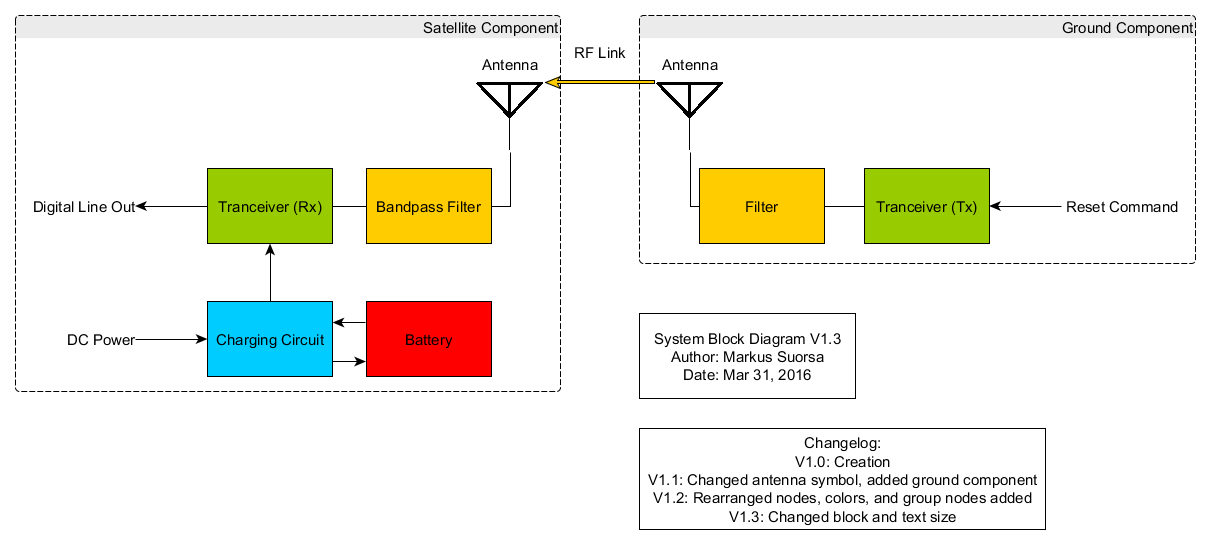
\includegraphics[scale=0.5]{blockdiagram}
\label{blockdiagram}
\end{sidewaysfigure}

\end{document}
